The following chapter will describe the concepts and reasons behind various components needed to allow a broker to
leverage modern reinforcement learning tools in the \ac {PowerTAC} environment. Current state-of-the-art
algorithms for \ac {RL}, available in Python \citep{baselines}, are used. These leverage both the TensorFlow library and, in one project, the Keras high-level abstraction library \citep{plappert2016kerasrl}. 

In general, a considerable amount of work was invested enabling communication between an agent
written in Python and the \ac {PowerTAC} systems which are Java based. The preliminary research and its results are summarized in
Section~\ref{sec:connecting_python_agents_to_powertac}. Because of this additional complexity, the practical part of the thesis was
restructured to allow for successful contribution to the \ac {RL} field by performing a form of \emph{what-if} 
analysis in the wholesale market which is described in Section~\ref{sub:wholesale_market}. The Python environment has
been constructed in a way to allow for future developers to leverage it as a framework for developing a fully capable
agent that acts in all markets. 

The overall architecture for the agent is composed of three key modules.First, the environment module, which hosts all known
information about the environment of the broker. This is used by all learning components. Second, A communication module
bridges the environment module and the \ac {PowerTAC} environment to hide communication overhead from the agent code,
letting the learning components access the environment as if it was not remotely defined.
Third, the agent components module holds all learning components such as the wholesale trader, the demand estimator
and the tariff manager. In the scope of this thesis, only the demand estimator and the wholesale trader were implemented
but the framework allows for the additional components to be easily implemented. The architecture is visualized in
Figure~\ref{fig:agentframework}. 

\begin{figure}[]
    \centering
    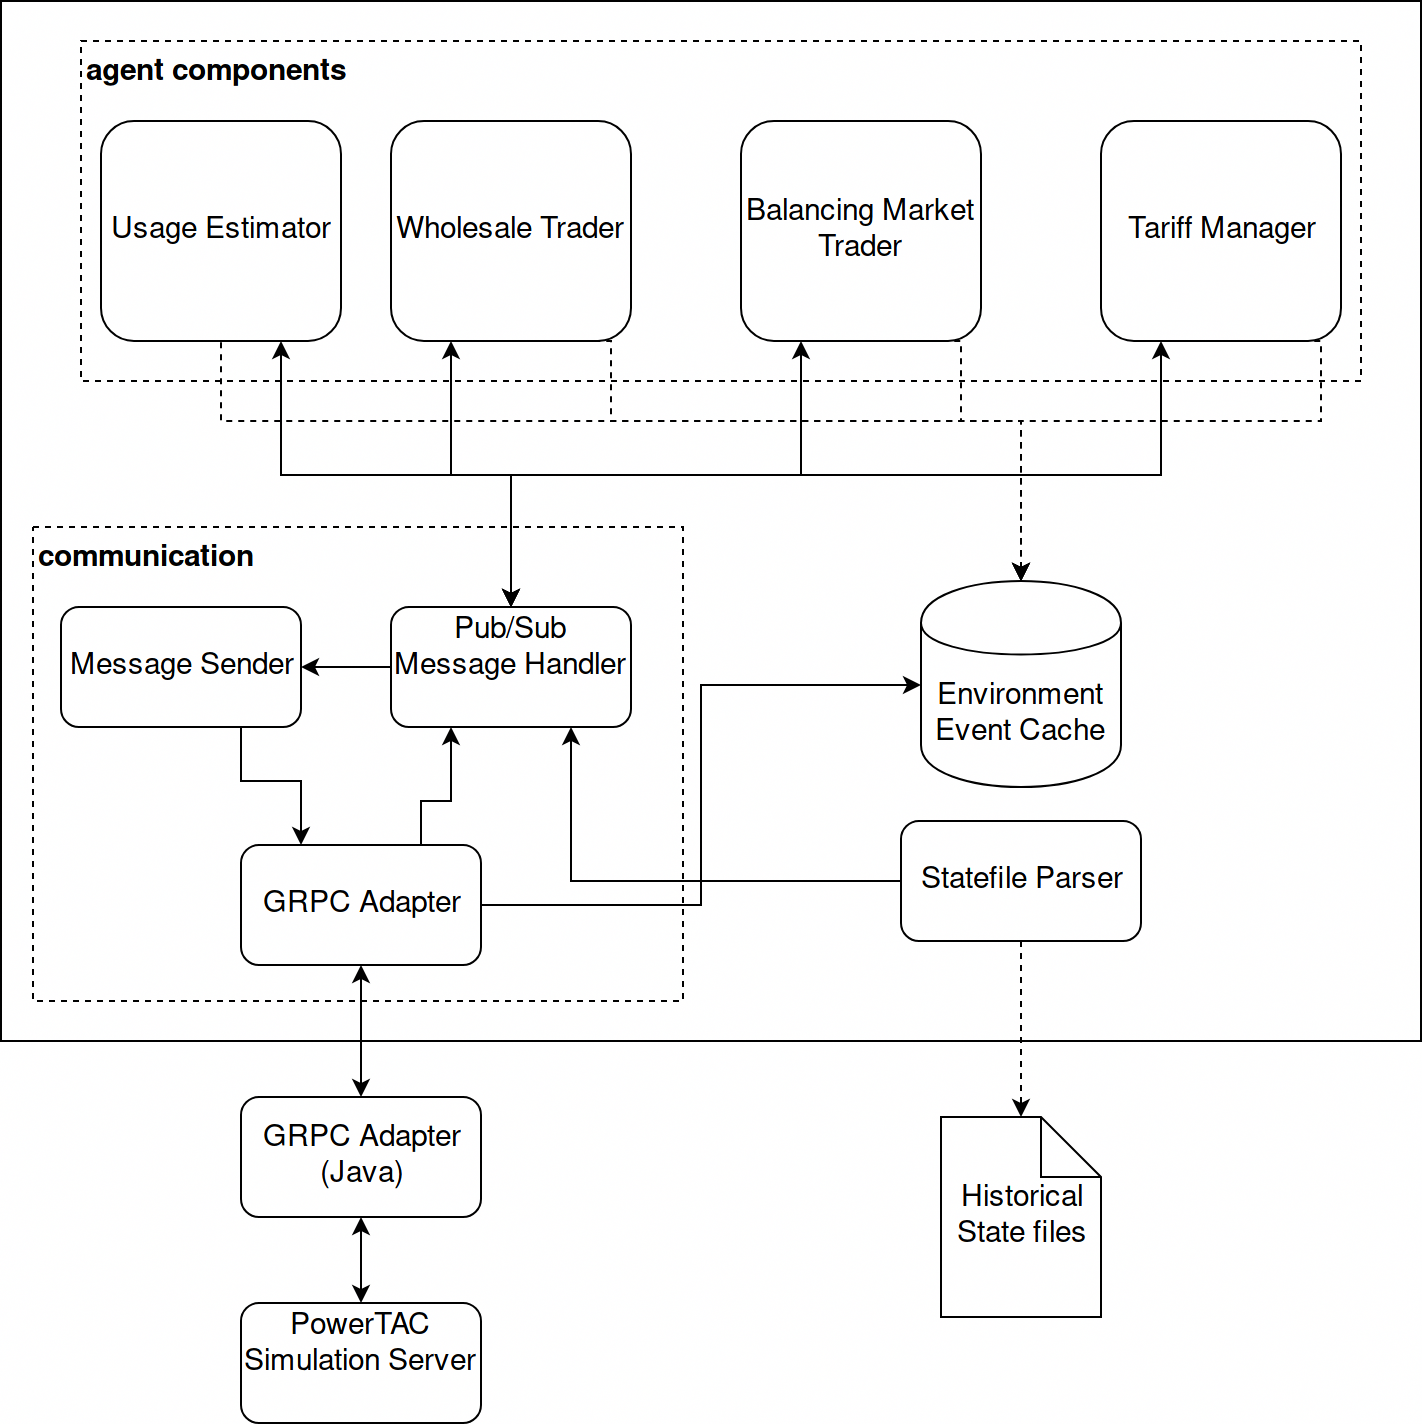
\includegraphics[width=0.8\linewidth]{img/Agent.png}
    \caption{Broker framework for Python}
    \label{fig:agentframework}
\end{figure}

\section{Tools}

To develop the functionality of the agent, which is supposed to be mainly driven by deep learning technologies, a number
of state-of-the-art tools and frameworks were  used. These include 
Keras and TensorFlow to allow for easy creation and adaption of the learning models, 
\ac {GRPC} to communicate with the Java components of the competition and
\emph{Click} to create a CLI interface that allows the triggering of various components of the broker.

%TODO IF Kubernetes is used, I need to complete it. But what about CRIU?
%Kubernetes to easily scale several instances across the cloud. 
%By transfering the components into the cloud, it is also
%possible to use tools such as Google Colab which allows access to a powerful cloud \ac {GPU} without costs
%\citep[]{GoogleColabOnline2018} .%TODO remove Google Inc in brackets


\subsection{TensorFlow and Keras}%
\label{sub:tensorflow_and_keras}

TensorFlow is a library developed by Google to facilitate machine learning algorithms. It can leverage both \ac {CPU}
and \ac {GPU} computing power which can significantly increase performance. It is Open Source, used in various
technologies and serves as a base technology for many higher level frameworks \citep{tensorflow2015-whitepaper}.

Keras is one of these higher level frameworks that focuses on \ac {NN}. It offers a intuitive \ac{API}, oriented towards
\ac {NN} terminology, to quickly develop and iterate on various \ac {NN} architectures. It integrates TensorFlow and its
accompanying UI Tensorboard, which visualizes training, network structure and activation patterns. It also supports
other base technologies beside TensorFlow, but these will not be discussed. A simple example for a 2 layer Dense \ac
{NN} written in Keras is shown in Listing~\ref{lst:kerasbasic}.


\begin{listing}
\begin{minted}[linenos,numbersep=5pt,frame=lines,framesep=2mm]{python}
from keras.layers import Dense

model.add(Dense(units=64, activation='relu', input_dim=100))
model.add(Dense(units=10, activation='softmax'))
model.compile(loss='categorical_crossentropy',
              optimizer='sgd',
              metrics=['accuracy'])
# x_train and y_train are Numpy arrays -- just like Scikit
model.fit(x_train, y_train, epochs=5, batch_size=32)
loss_and_metrics = model.evaluate(x_test, y_test, batch_size=128) 
\end{minted}
\caption{Basic Keras 2 layer dense NN example}
\label{lst:kerasbasic}
\end{listing}

\subsection{Click}%
\label{sub:click}

Click allows the creation of CLI interfaces in Python. Programms can be customised with parameters and options as well
as structured into subcommands and groups \citep{clickcli}. This allows for patterns such as \mint{bash}|agent compete
--continuous| or \mint{bash}|agent learn demand --model dense --tag v2| An annotated function is shown in
Listing~\ref{lst:click_sample}.

\begin{listing}[h]
\begin{minted}[linenos,numbersep=5pt,frame=lines,framesep=2mm]{python}
@cli.command()
@click.option('--continuous', default=True)
def compete(continuous):
    """take part in a powertac competition"""
    import communication.powertac_communication_server as server
    server.serve()
\end{minted}
\caption{Click sample declaration}
\label{lst:click_sample}
\end{listing}

\subsection{CRIU}%
\label{sub:criu}
\ac{CRIU} allows the freezing and storage of an application during runtime. This permits what is an equivalent of a fork
of the \ac {PowerTAC} simulation in a given point in time. Because \ac{CRIU} is also integrated into Docker, creating
containers for various components of the competition (i.e. server and brokers) and freezing all of them in a coordinated
manner is very helpful. This allows for two "what if" scenarios to play out at a given point in time where the results
can be compared \citep{criu}. A typical scenario for the technology is the live migration of running applications across
server infrastructures. In theory, a checkpoint of an application allows the perfect recreation of the application state
even after a complete reboot of the machine or the moving of the application to a different host with identical
environment settings.  

\subsection{Docker}
\label{sub:docker}

Docker allows to create isolated, transferable images that include everything an application requires to run. A
container can be based on various distributions and many containers can run on a single server without much overhead.
\ac{VM} technologies are often compared to containers, but \ac{VM}s abstract on a different layer. A \ac{VM} simulates
an entire operating system on top of a layer called the hypervisor. Docker on the other hand only abstracts the
application layer, letting all containers run in the same kernel and therefore makes use of the existing ressources in a
more efficient way. Because \ac{CRIU} is integrated into Docker
\footnote{at the time of writing, CRIU support is experimental in Docker},
containers can be stored to disk using the \emph{checkpoint} feature. 

\section{Preprocessing}

To learn from the large amount of data already available from previous simulations, parsing the state files provided by
the simulation is a reasonable approach to boost the ability of several parts of the agent to learn faster. One example
is the predictor of customer energy usage, as previous simulations offer large amounts of usage data that can be
analyzed.

The general architecture of the agent follows the idea of a core \emph{environment} module that holds all relevant data
for a game. Tariffs, rates, customers, transactions and other data is stored in this module. Since the state files are
based on events (they hold constructor parameters and method call parameters of previous server instances), these events
need to be translated into the environment. To learn from these events, most modern frameworks require a training
data-set and a label data-set. Therefore these events are first translated into an environment and at each timestep,
relevant training samples are extracted. Therefore the overall structure of the translation from state files to training
data is as follows:

\begin{enumerate} \item Iterate over all local state files \item Iterate over lines in state file \item Apply line to
current environment state \item At each time-step, extract relevant samples \item Store training data in separate local
files \end{enumerate}

The code linked to the process described above is part of the \texttt{util.state\_extractor} and
\texttt{model.environment} modules. The tests in the \texttt{tests} module document the functionality.

After the translation, the data is usually structured in a multi-dimensional array which can be read by numpy and
processed with Keras. First, some preprocessing can be applied with scikit-learn to analyze the structure of the data as
well as ensure the values that are fed to the \ac {NN} don't negatively impact the learning progress. The overall
approach follows the recommendations of \citep{Goodfellow-et-al-2016}.  


\section{Connecting Python agents to PowerTAC}%
\label{sec:connecting_python_agents_to_powertac}



To connect an agent based on Python to the \ac{PowerTAC} systems, a new adapter needs to be developed. In 2018, a simple
bridge was provided by the team that allowed external processes to communicate with the system through a bridge via the
provided sample-broker. All messages received by the broker are written to a First in First Out pipe on the local file
system and a second pipe is created to read messages from the external process. This was the first approach towards
opening up the simulation to other languages and development environments. 

As I am interested in writing my Agent using certain frameworks which are mainly developed and maintained in Python and
because it is helpful to also allow access to the adapter via network interfaces (to allow for distributed execution of
the components in e.g. cloud environments), I need to adapt this to allow network based access. In general the following
problems need to be solved:

\begin{itemize} \item Java model classes should be reused if possible, automatically generating target language model
	definitions from the Java source code to avoid duplication of semantically identical information \item Permit
	future developers using even more languages (such as C, R or Go) with little effort \item Possibly lay the basis
	for a change of the communication technology of the entire simulation which is more language agnostic.
	\end{itemize}

The first approach is based on \ac{GRPC} to transmit the messages between the Java sample-broker and the final client.
For this, each \texttt{handleMessage} method in the three core classes of the sample-broker passes the received message
along to the \ac {GRPC} infrastructure. While previous developers have handled these messages in the Java environment, I
pass these messages to the ultimate environment by converting them into protobuf messages which are then sent to a
connected broker who implements correpsonding handler methods in the target language. The advantage of this approach is
that this theoretically allows the maintainers of the project to also adapt this approach the Java clients in general,
which would then allow the makeshift Java \emph{bridge} to be avoided. The over-the-wire protocoll is also much more
efficient (as the data is sent in a binary format) and the message structre is clearly documented in the
\texttt{grpc\_messages.proto} file. The disadvantage is the need to translate each \ac{POJO} into a protobuf message and
vice versa. This is however not different from the current XStream implementation which also requires the annotation of
class files in Java to declare which properties are serialized and included in the \ac {XML} strings. If th project
should adopt the \ac {GRPC} based communcation, the \ac {GRPC} architecture will then allow the server to be adressed by
any of the supported languages.  \footnote{Which as of today are: C++, Java, Python, Go, Ruby, C\#, Node.js, PHP and
Dart}

A second approach is quiet similar to the original bridge but instead of writing the \ac {XML} strings to the local file
system, they are passed to the final environment via \ac {GRPC} by simple messages that just serve as a wrapper for the
\ac {XML} string. While this is not elegant from a engineering perspective (\ac {GRPC} should be used on a method level
and messages should not contain other message formats as strings), it is simple and may lead to quick results. A problem
is that the resulting \ac {XML} will then have to be parsed in the Python broker. Before the introduction of other
languages, the communication was basically an internal API and broker developers only needed to concern themselves with
the handling of the Java \texttt{handleMessage} method . Therefore, no formal descriptions for the structure of the \ac
{XML} messages exist. All \ac {XML} parsing would therefore be based on observable structures of the \ac {XML} which can
be extracted from the sample-broker logs and all model classes need to be rewritten. Furthermore, agents wanting to use
other programming languages would have to reimplement all of this again, with no core reuse possible.

A final approach is the generation of schema definitions from the Java model classes that are transmitted between the
brokers and the server. Generally, two human readable over-the-wire structures are reasonable: \ac {XML} and \ac{JSON}.
\ac {XML} messages can be formally defined using \ac {XML} Schemas and the \ac{JAXB} project
\footnote{\url{https://github.com/javaee/jaxb-v2}} offers to generate such schemas from Java class definitions. This
however did not succeed for the \ac {PowerTAC} model definitions which lead me to create a question on StackOverflow, a
discussion platform for programming questions. The resulting answer lead to the ultimate alternative which is the
generation of \ac {JSON} schemas which can then be converted into Python class files
\footnote{\url{https://stackoverflow.com/questions/49630662/convert-java-class-structures-to-python-classes/49777613\#49777613}}.
The choice of \ac {JSON} as the base communication protocoll might also be intelligent as a future choice two reasons:
Firstly, it seems to be the more popular serialization protocol in comparison to \ac {XML} \citep{jsonxml} due to its
easy readability and because it is more data efficient. Secondly, \ac {GRPC} can also transmit data in \ac {JSON} form
and protobuf messages can easily be printed as \ac {JSON}, making both alternatives more interoperable
\footnote{\url{https://github.com/powertac/broker-adapter-grpc} }.

Because the programming language is different from the supplied sample-broker, many of the domain objects need to be
redefined and some code redeveloped. The classes in \ac {PowerTAC} which are transfered between the client and the
server are all annotated so that the xml serializer can translate between the xml and object variants without errors.
This helps to recreate a similar functionality for the needed classes in the python environment. If the project was
started again today, it might have been simpler to first define a set of message types in a language such as Protocoll
Buffers, the underlying technology of \ac {GRPC}, but because all current systems rely on \ac {JMI} communication, it is
better to manually recreate these translators. The \ac {XML} parsing libraries provided by Python can be used to parse
the \ac {XML} that is received.  

%\section{Parallelizing environments with Kubernetes}

\section{Using Docker to make the competition portable}%
\label{sec:using_docker_to_make_the_competition_portable}

To run a competition on a local machine, one must install several components: Maven, Java 8 and all of the brokers as
well as ones own technology stack. If the scale of this set of components exceeds the local computation power available,
the stack needs to be moved to a machine in a server with sufficient computation power. While tools like Vagrant allow
the configuration and setup of environments to quickly allow new developers to start working with a set of tools in a
given project \citep{vagrant} , it requires virtual machines which have significant overhead in comparison to container
technologies. If the competition is abstracted into docker images, tools like Kubernetes or Docker Compose can quickly
instantiate a competition on any machine, given it has enough resources and a docker runtime installed \citep{docker}.

To create a Docker image for the server, the \texttt{Dockerfile} listed in Listing~\ref{lst:servertodocker} can be used
\footnote{All resources regarding the container technologies can be found under \url{https://github.com/pascalwhoop/powertac-kubernetes}.  

\begin{listing}[h]
	
\begin{minted}[linenos,numbersep=5pt,frame=lines,framesep=2mm]{Dockerfile}
FROM openjdk:alpine
LABEL maintainer=pascalwhoop
LABEL name=powertac-server

#adding all the needed dependencies
RUN apk add --no-cache bash vim git maven python

#download the server-distribution from github
RUN mkdir data && \
	git clone https://github.com/powertac/server-distribution

#build once, saves all maven dependencies in image
RUN cd server-distribution && \
	mvn -Pcli

WORKDIR /powertac/server-distribution
COPY bootstrap-data.xml ./
COPY init.sh ./
COPY server.properties ./

EXPOSE 8080 61616
#and start it up
CMD /powertac/server-distribution/init.sh
\end{minted}
\caption{Turning the current server snapshot into a docker image}
\label{lst:servertodocker}
\end{listing}

The benefit of this: Tools like Kubernetes or Docker Swarm, both being open source enterprise level container management
software, seamlessly allow for the creation of 1, 10 or 1000 instances. OpenAI, a deep learning research company, has
successfully scaled Kubernetes to 2500 nodes to run their deep \ac{RL} learning systems \citep{openai2500}. As
previously mentioned, Docker also integrates \ac{CRIU} which is required for the creation of snapshots of competition
states.  

%TODO implement redis as base for communication between components
%\subsection{Redis and component messaging}%
%\label{sub:redis_and_messaging}


\section{Learning Components}
\label{sec:learning_components}
The components of the agent that have learning capabilities include: 

\begin{description} 
	%TODO will i still get to implement this? simply mimick an agents tariffs ... shouldn't be hard
	\item[Customer Market]: Generates actions in respect to the tariff market such as publishing,
	adapting and revoking tariffs. While the component is expected to have a positive impact on the performance of
	the broker, it was just implemented with a basic functionality of publishing the same tariffs as a selected
	competitive broker, mimicking the competing brokers portfolio. It also creates usage predictions for a set of
	customers for other components. Generally, the framework intends a tariff fitness evaluation as well as tariff
	selection component that weighs both competitiveness and expected profitability.  
	
	\item[Wholesale Market]: Places bids and asks for energy in the periodic double
	auction type market \citep{ketter2018powertac}. The component employs \ac {RL} techniques and uses the
	predictions generated from the customer market component as an input describing the required capacity.

	\item[Balancing Market]: The balancing market component has not been implemented, but it is part of the
	developed framework for possible future extension.  \end{description}

While \citep{tactexurieli2016mdp} have defined the entire simulation as a \ac {POMDP} (although they interpret it as a
\ac {MDP} for ease of implementation) with all three markets integrated into one problem, I believe breaking the problem
into disjunct sub-problems is a better approach as each of them can be looked at in separation and a learning algorithm
can be applied to improve performance without needing to consider potentially other areas of decision making. A
subsequent algorithm could then be trained to perform the same actions as one unified decision making system according
to the concepts of \emph{Curriculum Learning}\citep{matiisen2017teacher} and \emph{Transfer Learning}
\citep{parisotto2015actor}. Such a unified algorithm is not part of this work. 
To justify this separation of concerns, I refer to the estimation of fitness for a given tariff in a given environment. A tariffs' competitiveness in a
given environment is independent of the wholesale or balancing trading strategy of the agent since the customers do not
care about the profitability of the agent or how often it receives balancing penalties. While the broker might incur
large losses if a tariff is too competitive (by offering prices that are below the profitability line of the broker),
such a tariff would theoretically be quiet competitive and should therefore be rated as such. The question which of the
tariffs to actually offer on the market is a separate problem, that balances competitiveness against profitability.

\subsection{Tariff Market}

The goal of the customer market is to get as many subscribers as possible for the most profitable tariffs the broker
offers on the market. The tariffs offered in the market compete for the limited number of customers available and every
customer must be subscribed to some tariff. The profitability of tariffs is limited by the base tariff which is offered
by the simulation as a constant offering creating an upper bound on profitability. 

To succeed in the customer market, the agents needs to be able to generate tariffs that are competitive. This can be
broken down into two subtasks: Generating valid tariffs and evaluating their competitiveness. A tariff can be verified
by passing it to the \ac {PowerTAC} server which verifies the tariff. Hence, a \ac {RL} algorithm that is tasked with
creating competitive tariffs can be given feedback by penalizing non-conclusive tariffs. An invalid tariff could be one
that contains overlapping rates leading to an ambivalent status. The competitiveness of a tariff depends not only on the
attributes of the tariff but also on the competition environment. If the broker only competes against the default
tariffs, even many mediocre tariff offerings would perform well. In an environment with many competitors on the other
hand, a tariff needs to be well designed to generate profits. 

The agents learning task for the customer market is therefore designed in the following way:

\begin{enumerate} \item Learning to evaluate a tariffs competitiveness in relation to the competitive environment
	through supervised learning on the historical state logs of previous competitions \item Running a \ac {RL}
	algorithm which learns to choose parameters for tariffs that are valid and profitable in a given environment
    %\item Learning to generate valid tariff specifications through a genetic algorithm strategy, penalizing invalid
	%tariffs %TODO really, I go genetic?
\end{enumerate}

%TODO not yet actually realized, still applicable?
\subsubsection{Tariff fitness learning} To learn the fitness of a tariff while considering its environment, supervised
learning techniques can be applied. To do this, features need to be created from the tariffs specifications and its
competitive environment. Similar work has been done by \citep{cuevas2015distributed} who discretized the tariff market
in four variables describing the relationships between the competitors and their broker.   

For my broker, because \ac {NN} can handle a large state spaces, I create a more detailed description of the
environment. I still have to ensure the number of input features is fixed though, so a simple copy of all competing
tariffs is not a valid input for the environment description. Instead I create the following features from the tariff
market:

\begin{description} \item[Average Charge per hour of week Timeslot]: According to \\
	\texttt{TariffEvaluationHelper.java}, customer models evaluate tariffs on an per-hour basis. This means they are
	very precise in the evaluation of potential tariff alternatives (before the application of an irrationality
	factor). Hence, a per-hour precision in the input is needed.  \item[Variance of Charge per hour of week
	Timeslot] Variance of the tariffs charges per each timeslot in a week among all competitors.  \item[Average and
	Variance of periodic payments] Description of the markets periodic payments landscape \item[Average and Variance
	of one-time payments] Description of the markets one-time payments landscape \item[Average and Variance of
	Up/Down regulation payments] 0 for tariffs without regulation capabilities \end{description}

Because the \ac {PowerTAC} simulation does not return profits of brokers on a per-tariff basis and because the reasons
for why a broker purchased a specific amount of energy on the wholesale market are not known, it is hard to put a
profitability value on a brokers tariff if said broker offers more than one tariff on the market. Therefore the
evaluation of the tariff does not include the profitability of the tariff but merely the competitiveness in regards to
the attractiveness of the offer from the perspective of the customers
% large space of decision variables / dimensions
%
% how to avoid overwhelming of agent? output layer must be fairly large. 
%
% time, energy, money, communication dimensions (and subdimensions)
\subsubsection{Customer demand estimation}% \label{ssub:customer_demand_estimation}

The simplest learning component is the demand estimator. This component has no dependencies onto the other learning
components and can easily be trained using historical data. This is due to the fact that the demand of a customer is
only dependent on variables that are already provided in the state files of previous simulations. A customer will not
use a different amount of energy if the broker implementation changes but all other variables (such as subscribed
tariff, weather etc.) remain equal .

To train a model that predicts the demand amounts of customers under various conditions, a dataset of features and
labels needs to be created. Because the model may also learn during the course of a running competition (allowing the
model to adapt to new customer patterns), a generator based structure should be preferred. This means that a generator
exists that creates $x, y$ pairs for the model to train on.

According to the simulation specification, the customer models generate their demand pattern based on their internal
structure, broker factors and game factors \citep[]{ketter2018powertac}. The preprocessing pipeline therefore generates
feature-label pairs that include: Customer, tariff, weather, time and demand information. The realized demand is the
label while all other components are part of the features that are used to train the model. The intuitive model class
for demand patterns prediction are \ac {RNN} due to the sequential nature of the problem \citep[]{EvalGRU2014}. However,
as will later be shown, the implementation of relatively shallow dense classic \ac {NN} also results in decent results. 

\begin{figure}[h] \centering 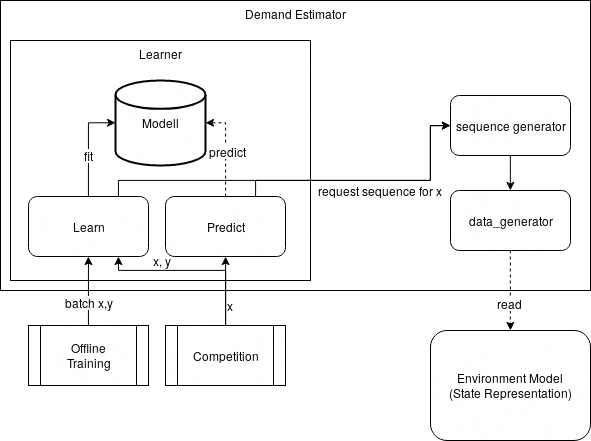
\includegraphics[width=0.8\linewidth]{img/UsageEstimator.png} \caption{Demand Estimator
structure} \label{fig:DemandEstimator} \end{figure}


The overall structure of the demand estimator component is shown in Figure~\ref{fig:DemandEstimator}. The model can be
both trained offline based on the state files as well as online during the competition. This is possible because in both
situations, the environment model of the agent is a continuous representation of the agents knowledge about the world.
In fact, during the state file parsing, the environment may even hold information that the agent usually cannot observe
in a competition environment. This is also the case for the demand learning, as the state files hold the demand
realizations of all customers while the server during the competition only transmits the usage realizations of the
customers that are subscribed to the agents tariffs. Regardless, this does not affect the ability to learn from the
customers usage patterns in either setting. During a competition, the agent may learn from the realized usage of
customers after each time slot is completed. Because this process may require some ressources, it is advantageous to
first perform the prediction of the subscribed customers demands for the current time slot to pass this information to
the wholesale component before training the model on the received meter readings \footnote{The component code can be
found under \url{https://github.com/pascalwhoop/broker-python/tree/master/agent_components/demand}}.


\subsection{Wholesale Market}
\label{sub:wholesale_market}



Using \ac {MDP} 

\ac {MDP} is actually with infinite states but for analytical concept, its irrelevant. Important is: Continuous states,
continuous actions (with some rounding to nearest .02)

Bellman equation not applicable to continuous spaces. But it is also unique because its a directed acyclic graph (the
state transition graph) 1, 2, 3, 4, ... 24

theoretically it's a nonstationary \ac {MDP} because it's limited to 24 state transitions before termination (t-0)

DQN --> evaluate the value of a s,a pair

\ac {PPO} --> use DNN for determining what to do in a given state - maximizes "surrogate" (relation between old and new
policy) while penalizing too extensive reward estimations (to avoid extensive updates to policy)

reward is based on relative price paid in comparison to average price for given time slot. 

Do I implement the env interface defined by OpenAI and let the agent subcomponent imagine it's by itself? --> allows for
A3C and many other interesting opportunities

